\documentclass[10pt]{beamer}
\usefonttheme{professionalfonts,serif}
\def\newblock{\hskip .11em plus .33em minus .07em}
\usepackage[numbers,sort]{natbib}
\renewcommand{\rmdefault}{psbx}
\usepackage[utf8]{inputenc}
\usepackage[T1]{fontenc}
\usepackage{textcomp}
\usepackage{eulervm}

\usetheme{default}           % tips from David Blei
\useinnertheme{circles}
\useoutertheme{infolines}
\setbeamertemplate{headline}{}
\setbeamertemplate{navigation symbols}{}
\setbeamerfont{itemize/enumerate subbody}{size=\normalsize}
\setbeamerfont{itemize/enumerate subsubbody}{size=\normalsize}
\usecolortheme{seahorse}
\setbeamersize{text margin left=2mm,text margin right=2mm}

\graphicspath{{../../figures/}}

\definecolor{mypine}{rgb}{0.05,0.45,0.05}
\definecolor{mycyan}{rgb}{0.0,0.9,0.9}
\newcommand{\Red}{\textcolor{red}}
\newcommand{\Blue}{\textcolor{blue}}
\newcommand{\Green}{\textcolor{mypine}}
\newcommand{\PineGreen}{\textcolor{mypine}}
\newcommand{\Magenta}{\textcolor{magenta}}
\newcommand{\Cyan}{\textcolor{mycyan}}

\newcommand{\N}{\mathcal{N}}
\newcommand{\R}{\mathbb{R}}
\newcommand{\T}{{\scriptsize^{\top}}}
\newcommand{\D}{\mathcal{D}}
\newcommand{\F}{\mathcal{F}}
\newcommand{\E}{\mathbb{E}}
\newcommand{\V}{\mathbb{V}}
\newcommand{\M}{\mathcal{M}}
\newcommand{\KL}{\mathcal{KL}}
\newcommand{\cut}[1]{}
\newcommand{\trace}{\operatorname{trace}}

\newcommand{\bmu}{{\boldsymbol{\mu}}}
\newcommand{\btheta}{\boldsymbol{\theta}}
\newcommand{\bepsilon}{\boldsymbol{\epsilon}}
\newcommand{\balpha}{\boldsymbol{\alpha}}
\newcommand{\bbeta}{\boldsymbol{\beta}}
\newcommand{\bphi}{\boldsymbol{\phi}}
\newcommand{\bPhi}{\boldsymbol{\Phi}}
\newcommand{\bSigma}{\boldsymbol{\Sigma}}
\newcommand{\bpi}{\boldsymbol{\pi}}
\newcommand{\blambda}{\boldsymbol{\lambda}}

\newcommand{\argmax}{\operatorname{argmax}}
\newcommand{\argmin}{\operatorname{argmin}}
\newcommand{\ci}{{\bot\negthickspace\negthickspace\bot}} % conditional indep.
\newcommand{\neigh}{\operatorname{ne}}
\newcommand{\vectr}[2]{  \left[ \!\!\begin{array}{c} #1 \\
      #2 \end{array} \!\!\right]}
\newcommand{\deff}{\stackrel{\mathrm{def}}{=}}
\newcommand{\deldel}[2]{\frac{\partial #1}{\partial #2}}

\newcommand{\maketilde}{\raisebox{0.4ex}{\tiny $\sim$}}
\newcommand{\bfa}{\mathbf a}
\newcommand{\bfb}{\mathbf b}
\newcommand{\bfe}{\mathbf e}
\newcommand{\bff}{\mathbf f}
\newcommand{\bfk}{\mathbf k}
\newcommand{\bfm}{\mathbf m}
\newcommand{\bfn}{\mathbf n}
\newcommand{\bfp}{\mathbf{p}}
\newcommand{\bfs}{\mathbf s}
\newcommand{\bfu}{\mathbf u}
\newcommand{\bfx}{\mathbf x}
\newcommand{\bfy}{\mathbf y}
\newcommand{\bft}{\mathbf t}
\newcommand{\bfv}{\mathbf v}
\newcommand{\bfw}{\mathbf w}
\newcommand{\bfA}{\mathbf A}
\newcommand{\bfI}{\mathbf I}
\newcommand{\bfK}{\mathbf K}


\title{Introduction to Text Modeling}
\author{Carl Edward Rasmussen}
\date{November 11th, 2016}

\begin{document}


\begin{frame}
\titlepage
\end{frame}


\begin{frame}
\frametitle{Key concepts}

\begin{itemize}
\item modeling document collections
\item probabilistic models of text
\item Zipf's law
\item bag of words representations
\end{itemize}
\end{frame}


\begin{frame}
\frametitle{Modelling text documents}

Here is an article from the Daily Kos (a US political blog) from
Feb 16 2014:

\begin{center}
\fbox{\parbox{0.9\textwidth}{\scriptsize \tt
GOP abortion foes are criminalizing the doctor-patient relationship\\

"The doctor-patient relationship." For more than 20 years,
conservative propagandists and their Republican allies have used that
four-word bludgeon to beat back universal health care reform. In 1994,
GOP strategist Bill Kristol warned that "the Clinton Plan is damaging
to the quality of American medicine and to the relationship between
the patient and the doctor." Kristol's successful crusade to derail
Bill Clinton's reform effort was greatly aided by future "death
panels" fabulist Betsy McCaughey, who wrongly warned that Americans
would even lose the right to see the doctor of their choice. Twelve
years later, President George W. Bush proclaimed, "Ours is a party
that understands the best health care system is when the
doctor-patient relationship is central to decision-making." \\

With the victory of Barack Obama in 2008, GOP spinmeister Frank Luntz
told Republicans obstructing the Affordable Care Act in Congress to
once again "call for the 'protection of the personalized
doctor-patient relationship.'" And during the 2012 campaign, the GOP
platform declared the party would "ensure the doctor-patient
relationship." \\
...
}}
\end{center}


Why would we model text documents?\\[1ex]

How could we model this document?
\end{frame}


\begin{frame}
\frametitle{Example: word counts in text}

Consider describing a text document by the frequency of occurrence of
every distinct word.\\[1ex]

The UCI \Blue{\emph{Bag of Words}} dataset from the University of California, Irvine. 
\footnote{\texttt{http://archive.ics.uci.edu/ml/machine-learning-databases/bag-of-words/}}\\
For illustration consider two collections of documents from this dataset:
\begin{itemize}
\item KOS (political blog --- \texttt{http://dailykos.com}): 
\begin{itemize}
\item $D=3,430$ documents (blog posts)
\item $n=353,160$ words
\item $m=6,906$ \Blue{\emph{distinct}} words
\end{itemize}
\item NIPS (machine learning conference --- \texttt{http://nips.cc}): 
\begin{itemize}
\item $D=1,500$ documents (conference papers)
\item $n=746,316$ words
\item $m=12,375$ \Blue{\emph{distinct}} words
\end{itemize}
\end{itemize}
\end{frame}


\begin{frame}
\centerline{
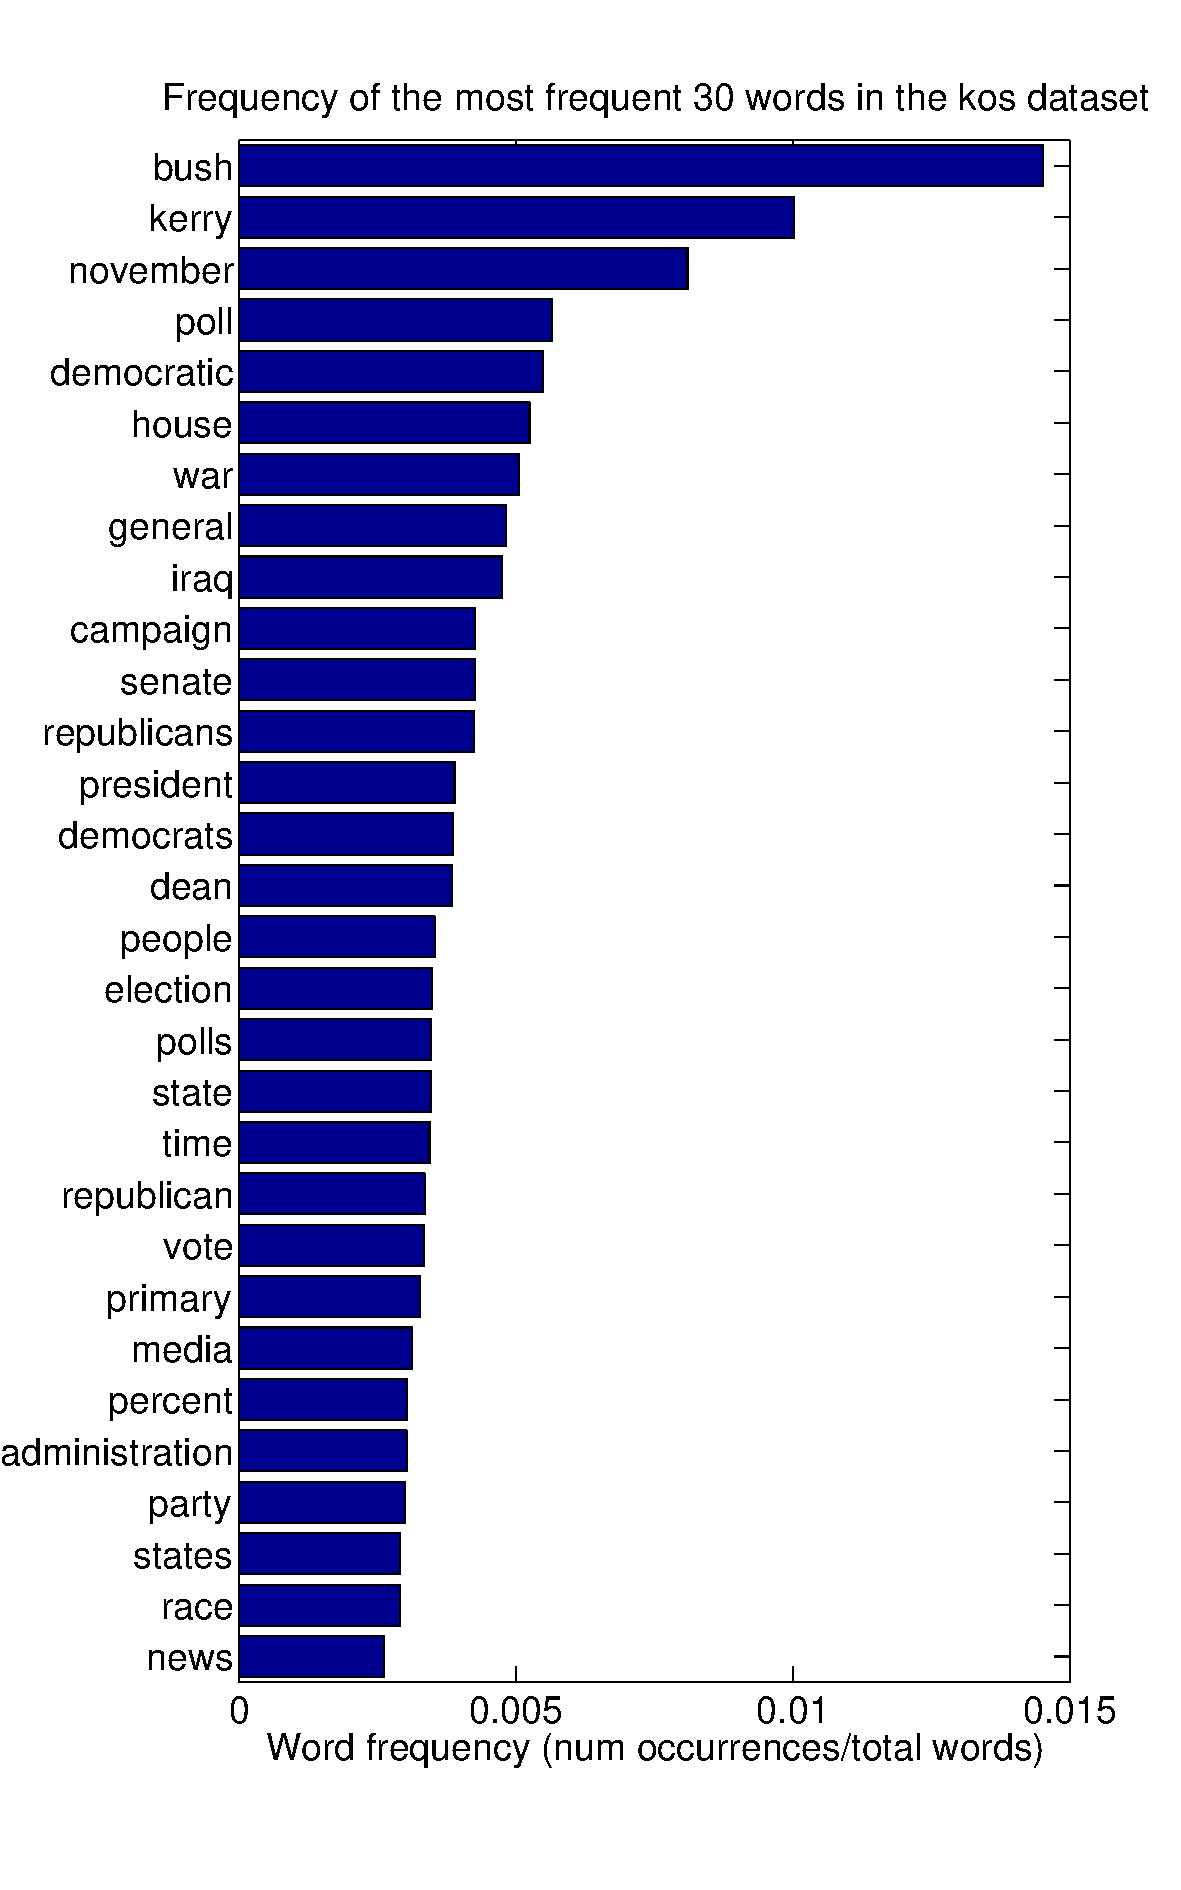
\includegraphics[width=0.5\textwidth]{kos_word_frequency}
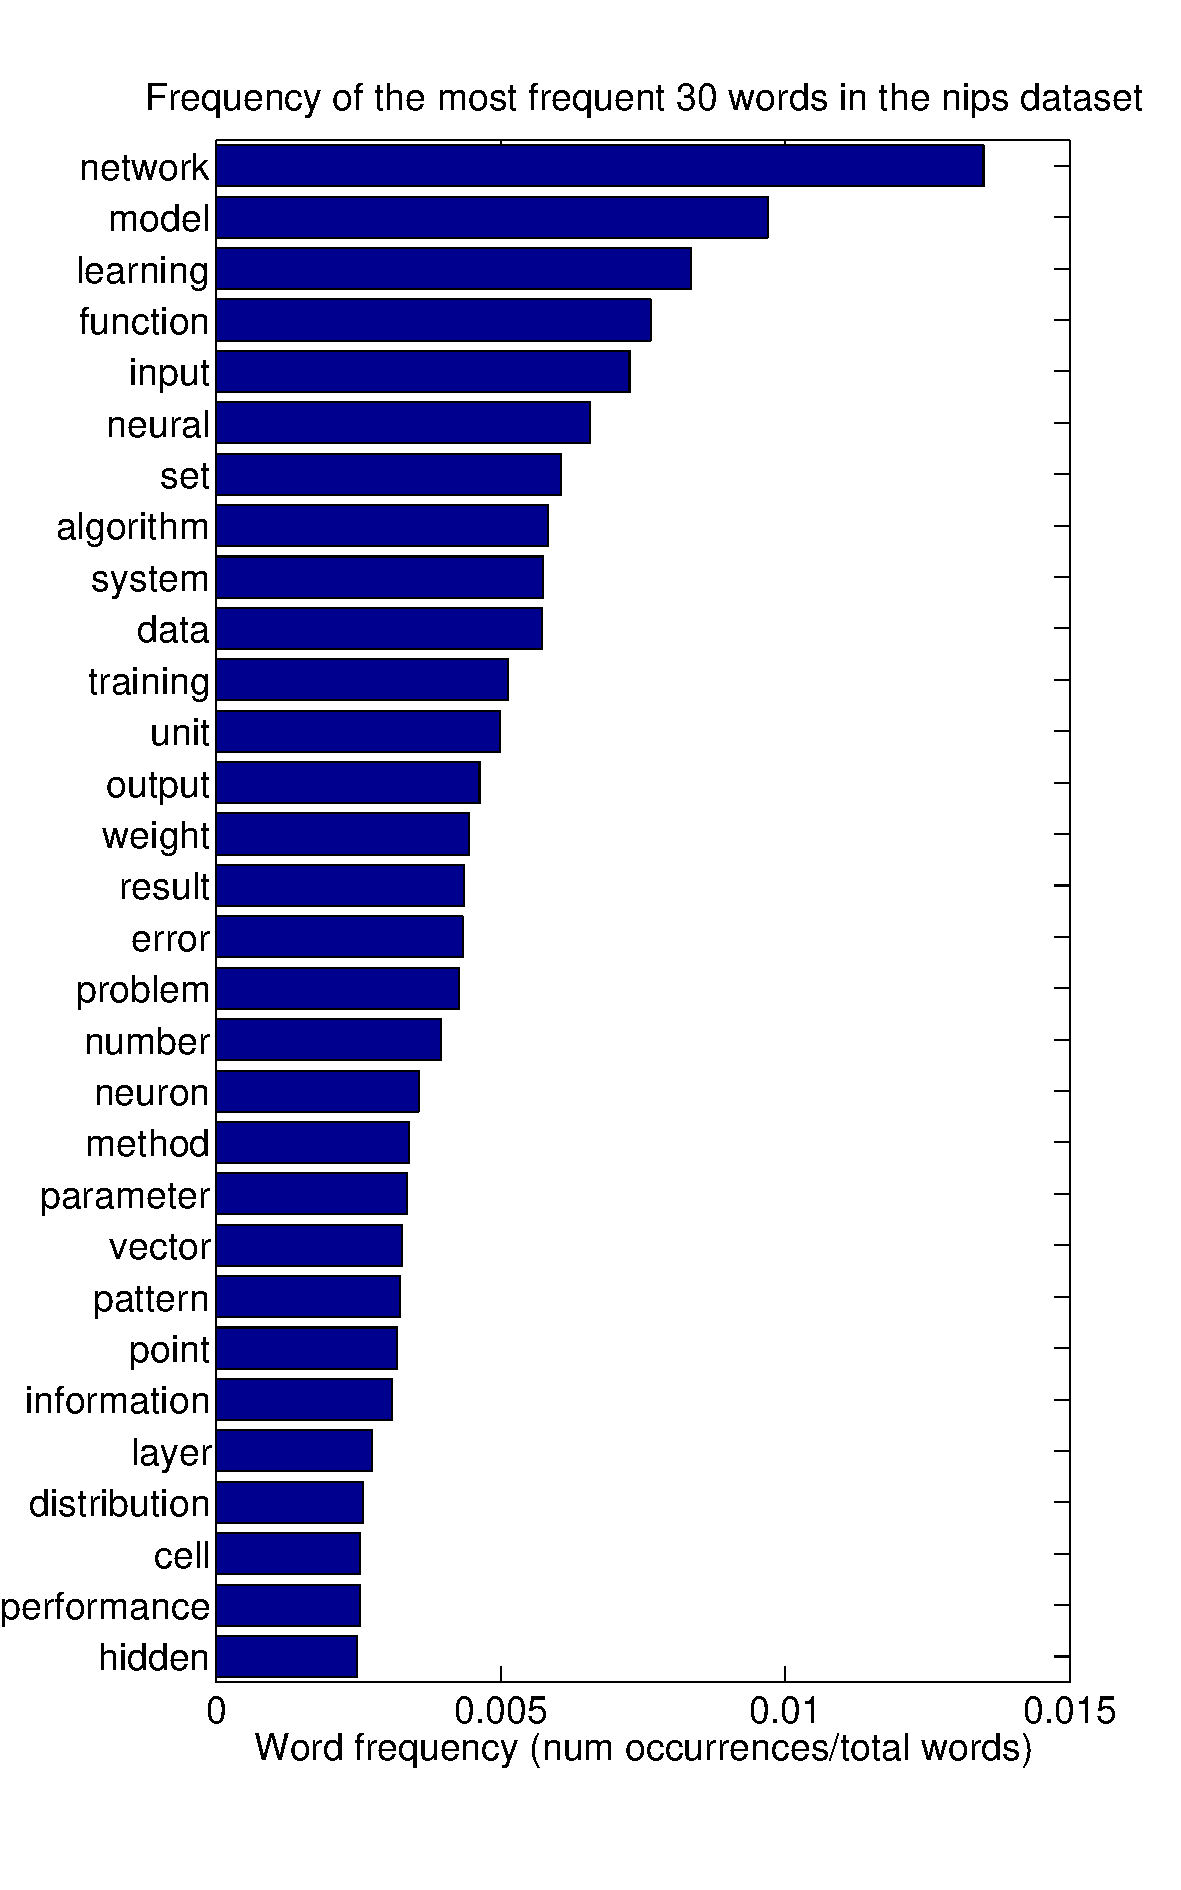
\includegraphics[width=0.5\textwidth]{nips_word_frequency}
}
\end{frame}

\begin{frame}
\frametitle{Different text collections, similar behaviour}

\centerline{
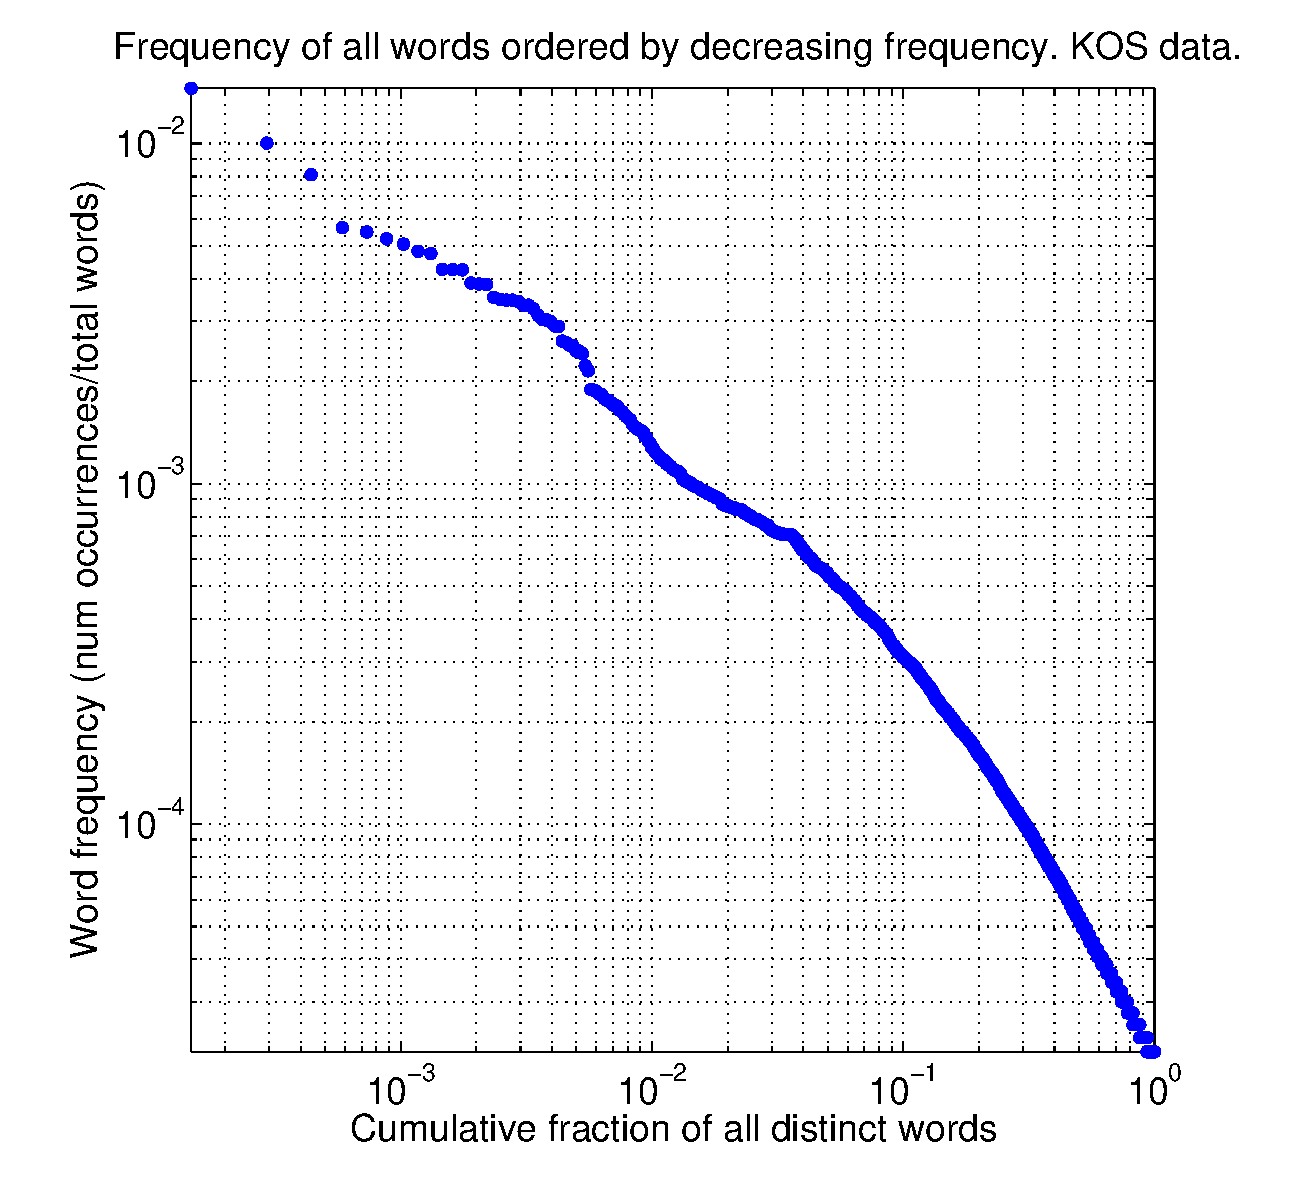
\includegraphics[width=0.5\textwidth]{kos_loglog_freqs}
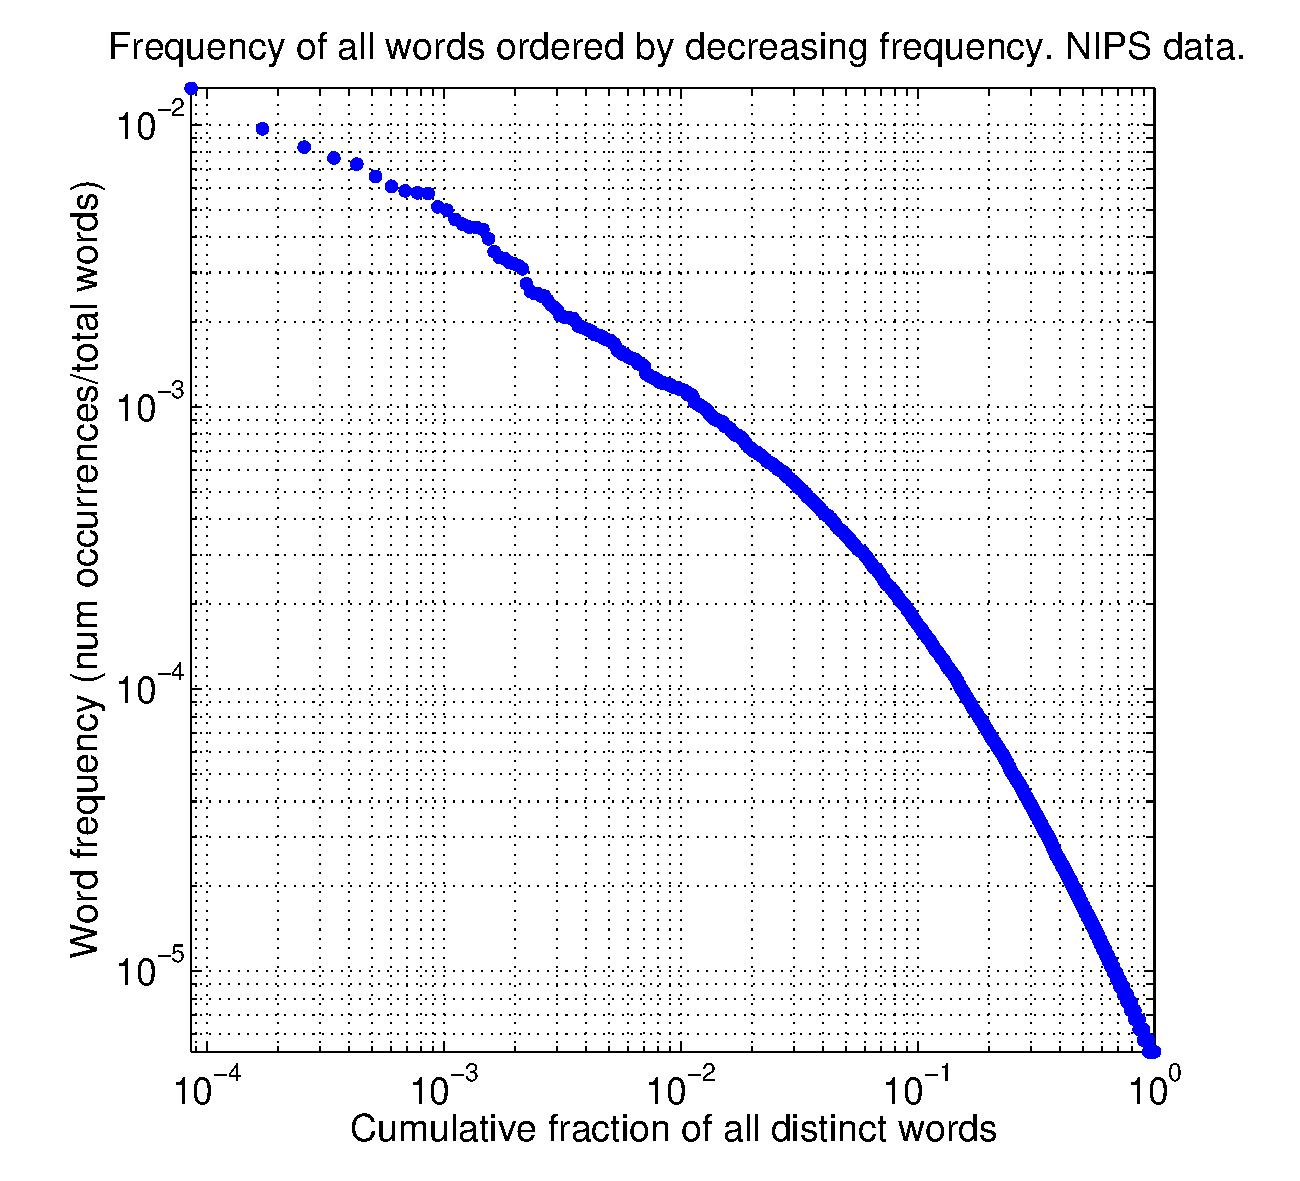
\includegraphics[width=0.5\textwidth]{nips_loglog_freqs}
}

Zipf's law states that \emph{the frequency of any word is inversely proportional 
to its rank in the frequency table}.
\end{frame}


\begin{frame}
\frametitle{Automatic Categorisation of Documents}

Can we make use of the \Blue{\emph{statistical distribution}} of words, to
build an automatic document categorisation system?

\begin{itemize}
\item The learning system would have to be \Blue{\emph{unsupervised}}
\item We don't \emph{a priori} know what categories of documents exist
\item It must \Blue{\emph{automatically discover}} the structure of
  the document collection
\item What should it even mean, that a document belongs to a category, or
  has certain properties?
\end{itemize} 

How can we design such a system?
\end{frame}

\end{document}